\documentclass[a4paper,12pt]{article}

\usepackage{graphicx} % Required for inserting images
\usepackage{amsmath,amssymb,amsfonts}
\usepackage{subcaption}
% Use Times New Roman font
\usepackage{times}
\usepackage[a4paper, top=1in, bottom=0.8in, left=1.1in, right=0.8in]{geometry}
\usepackage{float}
\usepackage{listings}
\usepackage{xcolor} % For customizing code colors
\setlength{\parindent}{0pt}
\usepackage{titlesec} % Add this to your preamble
\titleformat{\section}
{\normalfont\large\bfseries}{\thesection}{1em}{}
% Set spacing for sections
\titlespacing*{\section}
{0pt}  % Left spacing
{1ex} % Space before (adjust this value)
{1ex}  % Space after (adjust this value)
\begin{document}
	\section{Experiment No. 3}
	
	
	\section{Experiment Title }
	Design and Analyze 2 Input NAND and AND Gates Using1-Finger and 2-Finger MOS on
	MICROWIND 3.0
	\section{Objective}
	The main objectives of this report are:
	\begin{itemize}
		\item To design and simulate a CMOS inverter using MICROWIND 3.0.
		\item To ensure proper compliance with Design Rule Check (DRC) requirements during the design process.
		\item To design and simulate a tri-state inverter using MICROWIND 3.0
		\item To analyze the functionality and switching characteristics of both CMOS and tri-state inverters.
	\end{itemize}
	\section{Theory}
	\section{Schematic Layout }
	\section{Specification}
	\section{Output Waveshape }
	\section{Discussion }
	
\begin{figure}[H]
	\centering
	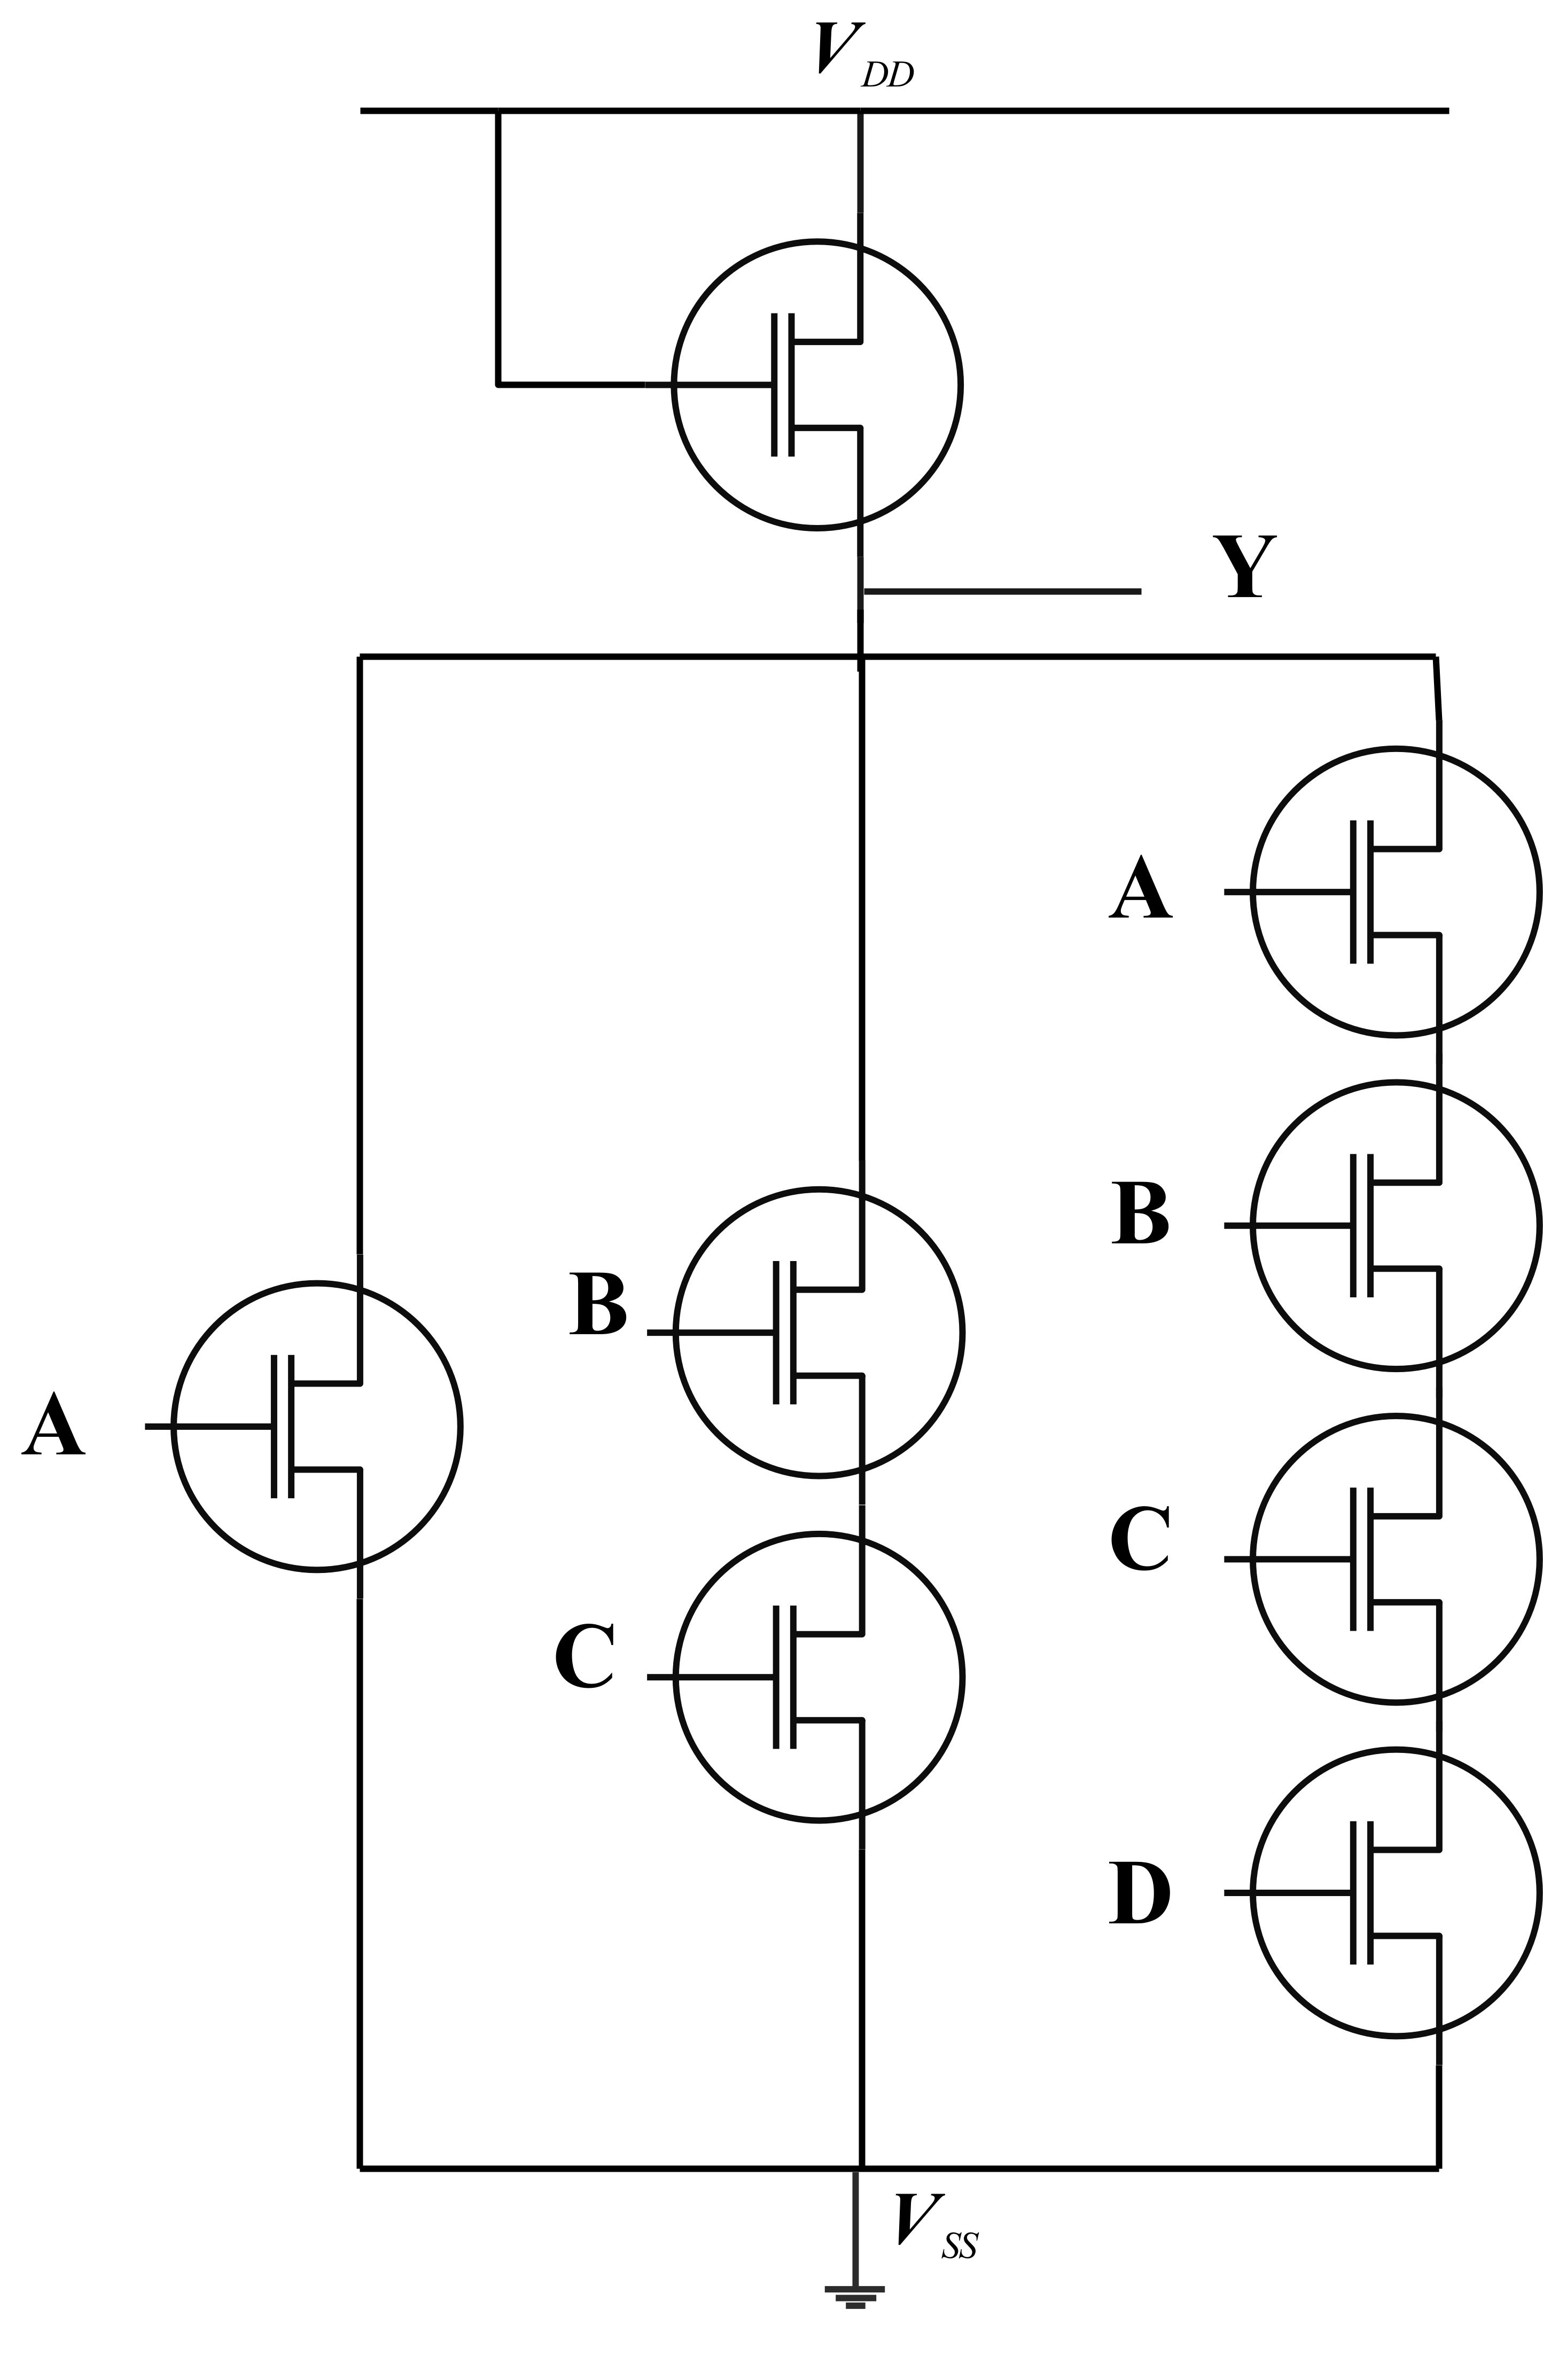
\includegraphics[width=0.7\linewidth]{Images/open}
	\caption{}
	\label{fig:open}
\end{figure}
	
\end{document}